\chapter{Technical Design}
\label{chap:technical}

\section{Architecture}

\begin{figure}[h] 
    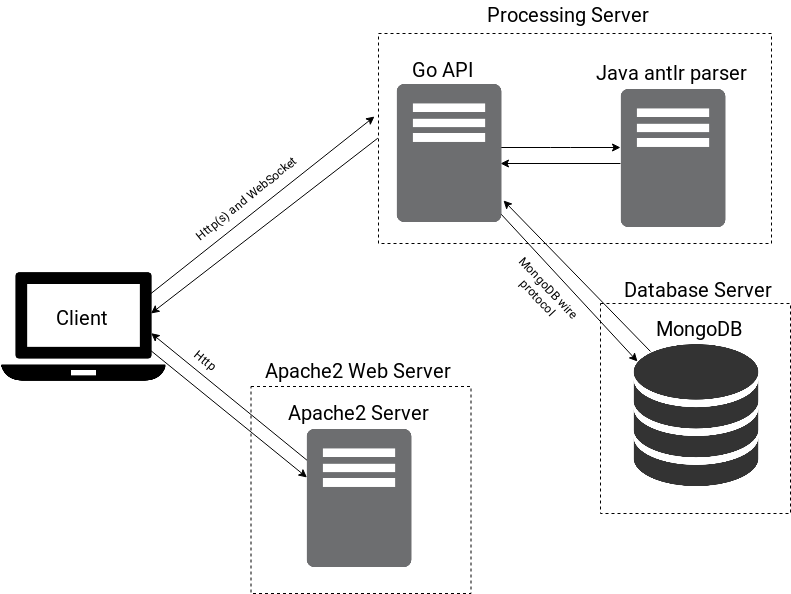
\includegraphics[width=\textwidth]{inc/images/CoVi_Architecture.png}
    \caption{System architecture.}
    \label{fig:architecture}
\end{figure}

\newacronym{api}{API}{Application Programming \Gls{interface}}
\newacronym{html}{HTML}{Hyper Text Markup Language}
\newacronym{css}{CSS}{Cascading Style Sheets}
\newacronym{http}{HTTP}{Hypertext Transfer Protocol}
\newacronym{antlr}{ANTLR}{ANother Tool for Language Recognition}
\newacronym{mvc}{MVC}{Model View Controller}
\newglossaryentry{server}{name=server, description={Computer in a network that is used to provide services  to other computers in the network}}
\newglossaryentry{client}{name=client, description={Computer in a network that uses the services provided by a \gls{server}}}
\newglossaryentry{js}{name=JavaScript, description={A "call by sharing" scripting language often used for \gls{client}-side web-applications}}
\newglossaryentry{websocket}{name=WebSocket, description={WebSockets is communication protocol, providing three communication channals; "Open", "Close", "Message" over a single transmission control protocol connection}}
\newglossaryentry{backend}{name=back-end, description={Back-end is the data access layer of a software}}
\newglossaryentry{Antlr}{name=Antlr, description={\gls{antlr} is a powerful parser generator for reading, processing, executing, or translating structured text or binary files. \cite{parr2013definitive}}}

As the figure \ref{fig:architecture} shows, the team divided the different components of the system. Initially the team had planned to implement the solution as a modern REST-full \gls{api}, where \gls{client} sends request to processing server for data to be handled. \Gls{client} uses \gls{http} and \glspl{websocket} to communicate with go \gls{api}, the reason \glspl{websocket} are used is because of lacking update on status of back-end processing for \gls{client} side.\glspl{websocket} can send multiple responses to the one sending request, this way we were able to show the status of processing to the \gls{client}.

Processing server consist of two components Go \gls{api} and Java antlr parser. Go \gls{api} is a REST-full \gls{api} but with some functionality implemented as \glspl{websocket}. Go \gls{api} is the common interface that \gls{client} communicate to store or receive data from the database server.Java \gls{antlr} parser is stand-alone helper application used by go \gls{api} to parse submitted project files. During implementation of the Java \gls{antlr} Parser, the team did some research to find the best way to use \gls{antlr} for parsing project files. Apache2 web server is used to send the \gls{html}, \gls{css} and \gls{js} to the \gls{client} through \gls{http} protocol. Database server is used by Go \gls{api} to update and fetch the data based upon \glspl{client} request.

\subsection{Front-end}
\newglossaryentry{interface}{name=interface, description={The means by which interaction or communication is achieved between systems}}
\newacronym{ui}{UI}{User \Gls{interface}}
\newglossaryentry{apache2}{name=apache2, description={A free and open-source cross-platform web server \cite{apacheServer}}}
\newglossaryentry{golang}{name=golang, description={Golang or Go is a statically typed compiled language in the tradition of C, with memory safety, garbage collection, structural typing, and CSP-style concurrent programming features added}}
\newacronym{fdg}{FDG}{Force Directed Graph}
\newacronym{loc}{LOC}{Lines Of Code}
\newacronym{json}{JSON}{\gls{js} Object Notation}
\newglossaryentry{namespace}{name=namespace,description={A named scope that prevents symbols from being mistaken for identically-named symbols in other scopes}}

\begin{figure}
\noindent\rule{\textwidth}{1pt}
\begin{lstlisting}[language=JavaScript, caption= {JSON structure from api}, label={lst:apiFormat}]
{
  "statuscode": 200,
  "statustext": "OK",
  "body":{
     "fileCount": 0,
     "id": "5cc9c475b7fa706ccb4700f1",
     "parsedFileCount": 0,
     "result": {
       "files": [
         {
           "parsed": false,
           "file_name": "5cc9c475b7fa706ccb4700f1/README.md",
           "linesInFile": 0
         },
         {
           "parsed": true,
           "file_name": "5cc9c475b7fa706ccb4700f1/main.cpp",
           "functions": [
             {
               "name": "main()",
               "declrator_id": "main",
               "return_type": "int",
               "function_body": {
                 "calls": [
                   {
                     "identifier": "printHelloWorld()",
                     "scopes": [
                       {
                         "identifier": "World",
                         "type": "namespace"
                       }
                     ]
                   }
                 ]
               },
               "start_line": 15,
               "end_line": 19
             }
           ],
           "namespaces": [],
           "linesInFile": 18
         }
       ]
     },
     "skippedFileCount": 0,
     "status": "Done"
  }
}
\end{lstlisting}
\noindent\rule{\textwidth}{1pt}
\end{figure}

The \gls{ui} form is given from a static \gls{apache2} server and populated by a dynamic \Gls{golang} server. The front-end consists of two separate parts; project info and code-base visualization.

The code-base visualization is where the functionality lies. It communicate with the \gls{api} to acquire a language independent representation of the code-base and getting parts of the code-base source. It expects the \gls{api} to serve \gls{json} in a similar format to listing \ref{lst:apiFormat}. The different parts of the response can be explained as below:
\begin{itemize}
    \item statuscode and statustext - Refers to a \gls{http} status to create a more uniform interface with \glspl{websocket} and normal \gls{http} requests.
    \item body - The requested data with what is required to represent the code-base and information on the completeness of the parsing.
    \item files - Represents a sourcefile in the repository
    \item functions, namespaces, classes, variable - Code blocks that the \gls{client} expect to contain code blocks for visualization
    \item call - A function call or assignment found in function code-block.
    \item scope - Shows if a call is executed on a variable.
\end{itemize}

Although what type of code-block can be within a type of code-block might depend on the language, the \gls{client} application allows for any code-block within any other and relies on the structure from the \gls{api} to be correct. This is done to make the application as language independent as possible.

The \gls{api} result is parsed to create the visualization with scopes, identifiers and relations. The representation is structured using a \gls{fdg} to space out separate structures with related structures close together and unrelated structures further apart. Each scope goes through the \gls{fdg} separately so to ensure that the scope is maintained in the representation whilst the scopes internal relations are based on the calls. The calls are connected to closest structure found to the function being called. The call might not always be connected to the actual function as the called function might be outside the repository or can not be identified due to the parser limitations. 

In addition the code-base visualization has a textual description of project metadata such as \gls{loc} and number of structures like \glspl{namespace}, classes and functions, that were found.

The project info part describes the project, refers to the \gls{git} repository  and describes the limitations of the program.

The limitations include unsupported browsers and limitations created by the incomplete parsing or unhandled code constructs.

\subsection{Back-end}
\label{sec:technicalBackEnd}
The processing server is the main server in \gls{backend}. It is responsible for handling the request from \gls{client} and send a response with a meaningful \gls{http} status code. Java \gls{Antlr} parser within the processing server is a stand-alone java application that uses \gls{Antlr} for language processing. \gls{Antlr} is a language recognition tool that uses a grammar file to assign a lexer token to each rule and then matches the token with a character sequence in the parsed file. \gls{Antlr} provides a listener for each rule in the grammar file. Once a rule matches a lexer token, it will callback to the respective listener. With this setup it became very straight forward to use \gls{Antlr} but it took a lot of time to understand the grammar files. Grammar files are created by different contributors which means names given for rules in the grammar are dependent on the contributor's choice and made it very hard for us to find rules for very specific language functionalities.

Go \gls{api} uses parts of \gls{mvc} pattern. \gls{mvc} pattern is widely used within web development because it excludes the coupling between \gls{ui} and logic. Go \gls{api} uses the model and controller parts of \gls{mvc} and view is managed by \gls{frontend}. Controller in go \gls{api} is responsible of handling validation, error handling and business logic whilst models represents abstraction of data model and encapsulates database handling.

Java \gls{Antlr} parser is designed to take in two arguments; file path and target language used in the file. In return Java \gls{Antlr} parser will output the parsed code in \gls{json} format to the standard output channel. The \gls{json} format was necessary so that parsed code would be uniformed for both C++ and Java targets. The parser takes only one file at a time so that Go \gls{api} could filter the project files that system does not support. This helped in limiting the \gls{Antlr} processing time.

As figure \ref{fig:sequenceInitial} shows, Go \gls{api} is responsible for handling requests from \gls{client}, validation, execution of Java \gls{Antlr} parser and handling database. For the initial request from user, Go \gls{api} will first check the database if project has been parsed previously and return the cached parsed code-base. If no caching has been done Go \gls{api} executes the Java \gls{Antlr} parser and passes the file to be parsed along with a target based on file's extension.

If the project to be parsed has multiple files Go \gls{api} will check what files of the project are supported by the Java \gls{Antlr} parser and will only send those files as an argument one at a time. Once the parser output is received in Go \gls{api}, it will construct and add the output  into project \gls{json}. Once all supported files are parsed, the project \gls{json} will be sent as a response to \gls{client}.

% talk about mvc and sequence diagram of initial request.
\begin{figure}[H] 
    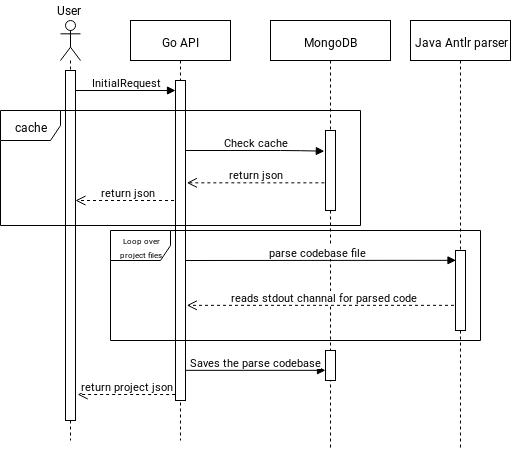
\includegraphics[width=\textwidth]{inc/images/InitialRequestSequenceDiagram.png}
    \caption{Sequence diagram of Initial request.}
    \label{fig:sequenceInitial}
\end{figure}

\subsection{WEB API}
\newacronym{uid}{UID}{Unique IDentifier}
% DRAFT!!!

At the start there was a requirement to have a REST-based \gls{api} to receive information about a given project. We therefore came up with the following structure:
\begin{itemize}
    \item /repo/add - Addition of a repository to the servers, this will, if it doesn't exist, clone it and return a new \gls{uid} else it returns the existing \gls{uid}.
    \item /repo/list - List all repositories that has been added to the server. So the user can see what's been parsed before.
    \item /repo/\{repoId\}/initial/ - The initial request used to fetch project structure and complexity measures. In the beginning this was a \gls{http}-method and since parsing a repository takes a long time, it could result in the user getting annoyed that no feedback on progress is returned. It was decided then that the initial \gls{api} endpoint would be upgraded to a web-socket that can maintain a connection and send multiple packets more naturally than basic \gls{http}-methods. This made us drift form the requirement of full a REST-based \gls{api} but to re-fulfill this requirement we could re-implement the original endpoint and serve it together with the web-socket.  
    
    The final result of the parsing is also cached for a quicker response, but the caching mechanics is every crude in the sense that it doesn't update the cached data even if the submitted repository has changed.
    \item /repo/\{repoId\}/file/read/ - Used to fetch any implementation at a specified location and size, in a given file.
\end{itemize}

A lot of focus was put on documentation, the group decided therefore to use \gls{api} Doc for this purpose. The generated documentation is hosted using an \Gls{apache2} web server. 